\documentclass[a4paper,12pt,openany,oneside]{book}
\usepackage[portuguese]{babel}
\usepackage[utf8]{inputenc}
%\usepackage[latin1]{inputenc}
\usepackage{indentfirst}
%\usepackage[T1]{fontenc}
\usepackage[final]{pdfpages}
\usepackage{lmodern}
\usepackage{epigraph}
\usepackage{hyperref}

\usepackage{lipsum}
\usepackage[usestackEOL]{stackengine}

%mudando o djabo do capitulo
%usando exemplo: https://pt.sharelatex.com/learn/Sections_and_chapters
\usepackage{titlesec}
 
\titleformat
{\chapter} % command
[display] % shape
{\bfseries\Large\itshape} % format
{Chapitre \ \thechapter} % label
{0.5ex} % sep
{
    \rule{\textwidth}{1pt}
    \vspace{1ex}
    \centering
} 


\setcounter{secnumdepth}{3}
% Pacotes ....................................................................................
% Pacotes Principais -----------------------------------------------------------
\usepackage[portuges,brazil]{babel}
\usepackage{ae} 
%%\usepackage[utf8]{inputenc}
%\usepackage[latin1]{inputenc}

%NO MAC ao inv�s de latin1 deve-se usar o applemac
\usepackage[applemac]{inputenc}

% Formatacaoo de capitulos ------------------------------------------------------
%\usepackage{capitulos}

% Figuras e Imagens ------------------------------------------------------------
\usepackage{graphicx}
% Figuras lado a lado
%\usepackage{epsfig} - REMOVIDO
%\usepackage{subfigure} - REMOVIDO

% Para poder ter tabelas com colunas de largura auto-ajust�vel
\usepackage{tabularx}

% Utilizar H para inserir as imagens REALMENTE onde eu desejo
%\usepackage{float} - REMOVIDO

% Para que os primeiros par�grafos das se��es tamb�m sejam indentados
% \usepackage{indentfirst} - REMOVIDO

%Permitir usar o comando \citeasnoun que coloca o nome na cita��o
\usepackage{harvard}


% Fontes -----------------------------------------------------------------------
%\usepackage[T1]{fontenc} - REMOVIDO
%\usepackage{pslatex} - REMOVIDO

% Matem�tico -------------------------------------------------------------------
%\usepackage{amsmath} - REMOVIDO
%\usepackage{amstext} - REMOVIDO

% Simbolos ---------------------------------------------------------------------
%\usepackage{textcomp} - REMOVIDO

% Tabelas ----------------------------------------------------------------------
%\usepackage{multirow} - REMOVIDO
% Colorir a tabela
%\usepackage{colortbl} - REMOVIDO

% Gloss�rio --------------------------------------------------------------------
%\usepackage[portuguese,noprefix]{nomencl}
%\usepackage{makeglo}

% Outros pacotes ---------------------------------------------------------------
%\usepackage{noitemsep} - REMOVIDO

%Subsubsection
%\usepackage{chngcntr} - REMOVIDO

% Para permitir espa�amento simples, 1 1/2 e duplo
\usepackage{setspace}

% Para executar um comando depois do fim da p�gina corrente
%\usepackage{afterpage} - REMOVIDO

% Para poder incluir arquivos Postscript com cores (do Xfig, por exemplo)
%\usepackage{color} - REMOVIDO

  % Itens numerados
%\usepackage{enumerate} - REMOVIDO

% Coment�rios em bloco
%\usepackage{verbatim} - REMOVIDO

% Refer�ncias ------------------------------------------------------------------
%\usepackage{html} - REMOVIDO
%\usepackage{url} - REMOVIDO
%\usepackage[abbr]{harvard}	% As chamadas s�o sempre abreviadas - REMOVIDO
%\harvardparenthesis{square}	% Colchetes nas chamadas - REMOVIDO
%\harvardyearparenthesis{round}	% Par�ntesis nos anos das refer�ncias - REMOVIDO
%\renewcommand{\harvardand}{e}	% Substituir "&" por "e" nas refer�ncias
%\renewcommand{\harvardurl}{URL: \url} - REMOVIDO

% Novos Comandos .....................................................................
% newcommand define novos comandos, que podem passar a ser usados da
% mesma forma que os comandos LaTeX de base.

% Configura��o da fonte
%\renewcommand{\familydefault}{\sfdefault}

% Margens ----------------------------------------------------------------------
%\setlength{\oddsidemargin}{3.5cm}
%\setlength{\evensidemargin}{2.5cm}
%\setlength{\textwidth}{15cm}
%\addtolength{\oddsidemargin}{-1in}
%\addtolength{\evensidemargin}{-1in}
%%
%\setlength{\topmargin}{2.0cm}
%\setlength{\headheight}{1.0cm}
%\setlength{\headsep}{1.0cm}
%\setlength{\textheight}{22.7cm}
%\setlength{\footskip}{1.0cm}
%\addtolength{\topmargin}{-1in}

% Cap�tulos --------------------------------------------------------------------
% N�o aparecer o n�mero na primeira p�gina dos cap�tulos
\newcommand{\mychapter}[1]{\chapter{#1}\thispagestyle{empty}}
\newcommand{\mychapterstar}[1]{\chapter*{#1}\thispagestyle{empty}}

% Os cap�tulos sem n�mero
%\newcommand{\mychapterast}[1]{\chapter*{#1}\thispagestyle{empty}
%\chaptermark{#1}
%\afterpage{\markboth{\uppercase{#1}}{\rightmark}}
%\markboth{\uppercase{#1}}{}
%}

%Referencias
%\newcommand{\BibTeX}{\textsc{B\hspace{-0.1em}i\hspace{-0.1em}b\hspace{-0.3em}}\TeX}

% Comandos matem�ticos ---------------------------------------------------------
% Implica��o em f�rmulas
%\newcommand{\implica}{\quad\Rightarrow\quad} %Meio de linha
%\newcommand{\implicafim}{\quad\Rightarrow}   %Fim de linha
%\newcommand{\tende}{\rightarrow}

% Fra��o com parenteses
%\newcommand{\pfrac}[2]{\parent{\frac{#1}{#2}}}

% Transformada de Laplace e transformada Z
%\newcommand{\lapl}{\pounds}
%\newcommand{\transfz}{\mathcal{Z}}

% Sequ�ncias
%\newcommand{\sequencia}[4]{$#1_{#2}$, $#1_{#3}$, \ldots, $#1_{#4}$}

% Se��es sem n�mero
%\newcommand{\mysectionast}[1]{\section*{#1}
%\addcontentsline{toc}{section}{#1}
%\markright{\uppercase{#1}}
%}

% No tabularx, as celulas devem ser centradas verticalmente
\renewcommand{\tabularxcolumn}[1]{m{#1}}

% C�lulas centralizadas horizontalmente no tabularx
\newcolumntype{C}{>{\centering\arraybackslash}X}


% Outros ----------------------------------------------------------------------
%\newcommand{\chave}[1]{\left\{#1\right\}}
%\newcommand{\colchete}[1]{\left[#1\right]}
%\newcommand{\parent}[1]{\left(#1\right)}

%%subsubsection
%\newcounter{subcount}
%\newenvironment{mysub}
%{\begin{list}
%{\textbf{\thesubsubsection.\arabic{subcount}}}
%{\setlength{\itemindent}{2.2em}
%\setlength{\rightmargin}{.6in}
%\setlength{\labelwidth}{1in}
%\setlength{\labelsep}{.2in}
%\setlength{\parsep}{.5ex plus .2ex minus .1ex}
%\setlength{\itemsep}{0ex plus .2ex minus 0ex}
%\usecounter{subcount}}
%}


%\citationmode{abbr}

% Inicia o texto
\begin{document}

% Paginas iniciais (sem numera��o)
\pagestyle{empty}

% P�gina de rosto (capa interna)
%
% ********** Pagina de Rosto
%

% titlepage gera paginas sem numeracao
\begin{titlepage}

\begin{center}

\small

% O comando @{} no ambiente tabular x é  para criar um novo delimitador
% entre colunas que não a barra vertical | que é normalmente utilizada.
% O delimitador desejado vai entre as chaves. No exemplo, não há nada,
% de modo que o delimitador é vazio. Este recurso está sendo usado para
% eliminar o espaço que geralmente existe entre as colunas
\begin{tabularx}{\linewidth}{ c X }
% A figura foi colocada dentro de um parbox para que fique verticalmente
% centralizada em relação ao resto da linha
\parbox[c]{7cm}{
\includegraphics[width=\linewidth]{polytech_logo}} &
\begin{center}
\textsf{\textsc{Polytech Nice Sophia\\ Analyse Conception Object
}} 
\end{center}

\end{tabularx}


% O vfill � um espa�o vertical que assume a m�xima dimens�o poss�vel
% Os vfill's desta p�gina foram utilizados para que o texto ocupe
% toda a folha
\vfill

\LARGE

\textbf{TD 2}

\vfill

\Large

\textbf{\href{mailto:gabicavalcantesilva@gmail.com}{CAVALCANTE DA SILVA Gabriela},\\
\href{mailto:cesar.colle@gmail.com }{COLLE César},\\\href{mailto:oliveira.raquel.lopes@gmail.com}LOPES DE OLIVEIRA,\\ \href{mailto:arnold.schweitzer@gmail.com}{SCHWEITZER Arnold}}

\vfill

\normalsize

Enseignant: Colette Michel

\vfill

\hfill
\parbox{0.5\linewidth}{\textbf{
A faire:} Diagranne UC (he haute niveau); Diagramme UC détailllés et Scéncarios Cockburn correspondant.}


\vfill

\large

%Data
Valbonne, FR, février 25

\end{center}

\end{titlepage}
  

%Espa�amento 1 1/2
\onehalfspacing  

\clearpage

% Paginas introdut�rias (com numera��o romana)
\frontmatter

%sResumo
\include{01_Introducao/resumo} 

% Lista de conte�do (sum�rio, gerado automaticamente)
%\addcontentsline{toc}{chapter}{Sumario}
%\renewcommand{\contentsname}{Sumário}
%\tableofcontents  
\begingroup
\let\cleardoublepage\clearpage
\renewcommand{\contentsname}{Plan}
\tableofcontents
\endgroup


% Lista de figuras (gerada automaticamente)
%\cleardoublepage 
%\addcontentsline{toc}{chapter}{Liste des Images}  
%\listoffigures  


% P�ginas do texto principal (com cabe�alho)
\mainmatter
\pagestyle{headings}

% Para facilitar a organiza��o, foi criado um diret�rio para cada
% cap�tulo do documento, pois assim os arquivos das figuras ficam
% classificados por cap�tulos
% Introdu��o

%\mychapter{Introduction}
%\mychapterstar{Introduction}
\chapter{Introduction}
\label{Cap:introduction}
Cette TD c'est pour delivrer une neuvelle version sur les activites sur le TD(1) et ajouter le premiere version sur le TD2 avec les : \textit{Diagramme UC de haut niveau)}, \textit{diagrammé UC détaillés}, \textit{Scenários Cockburn} sur le cas de use \textbf{passage} sur un péage autoroutier. 

% Desenvolvimento
%

\mychapter{Réécriture}
\label{Cap:TD1}


\section{Description physique}
Nous avons perçu que le système demandé sur la gestion d’une voie de péage d’autoroute.
%Nous avons élaborré dans ce document une première description de système d’un péage d’autoroute.

\begin{figure}[h]
    \centering
    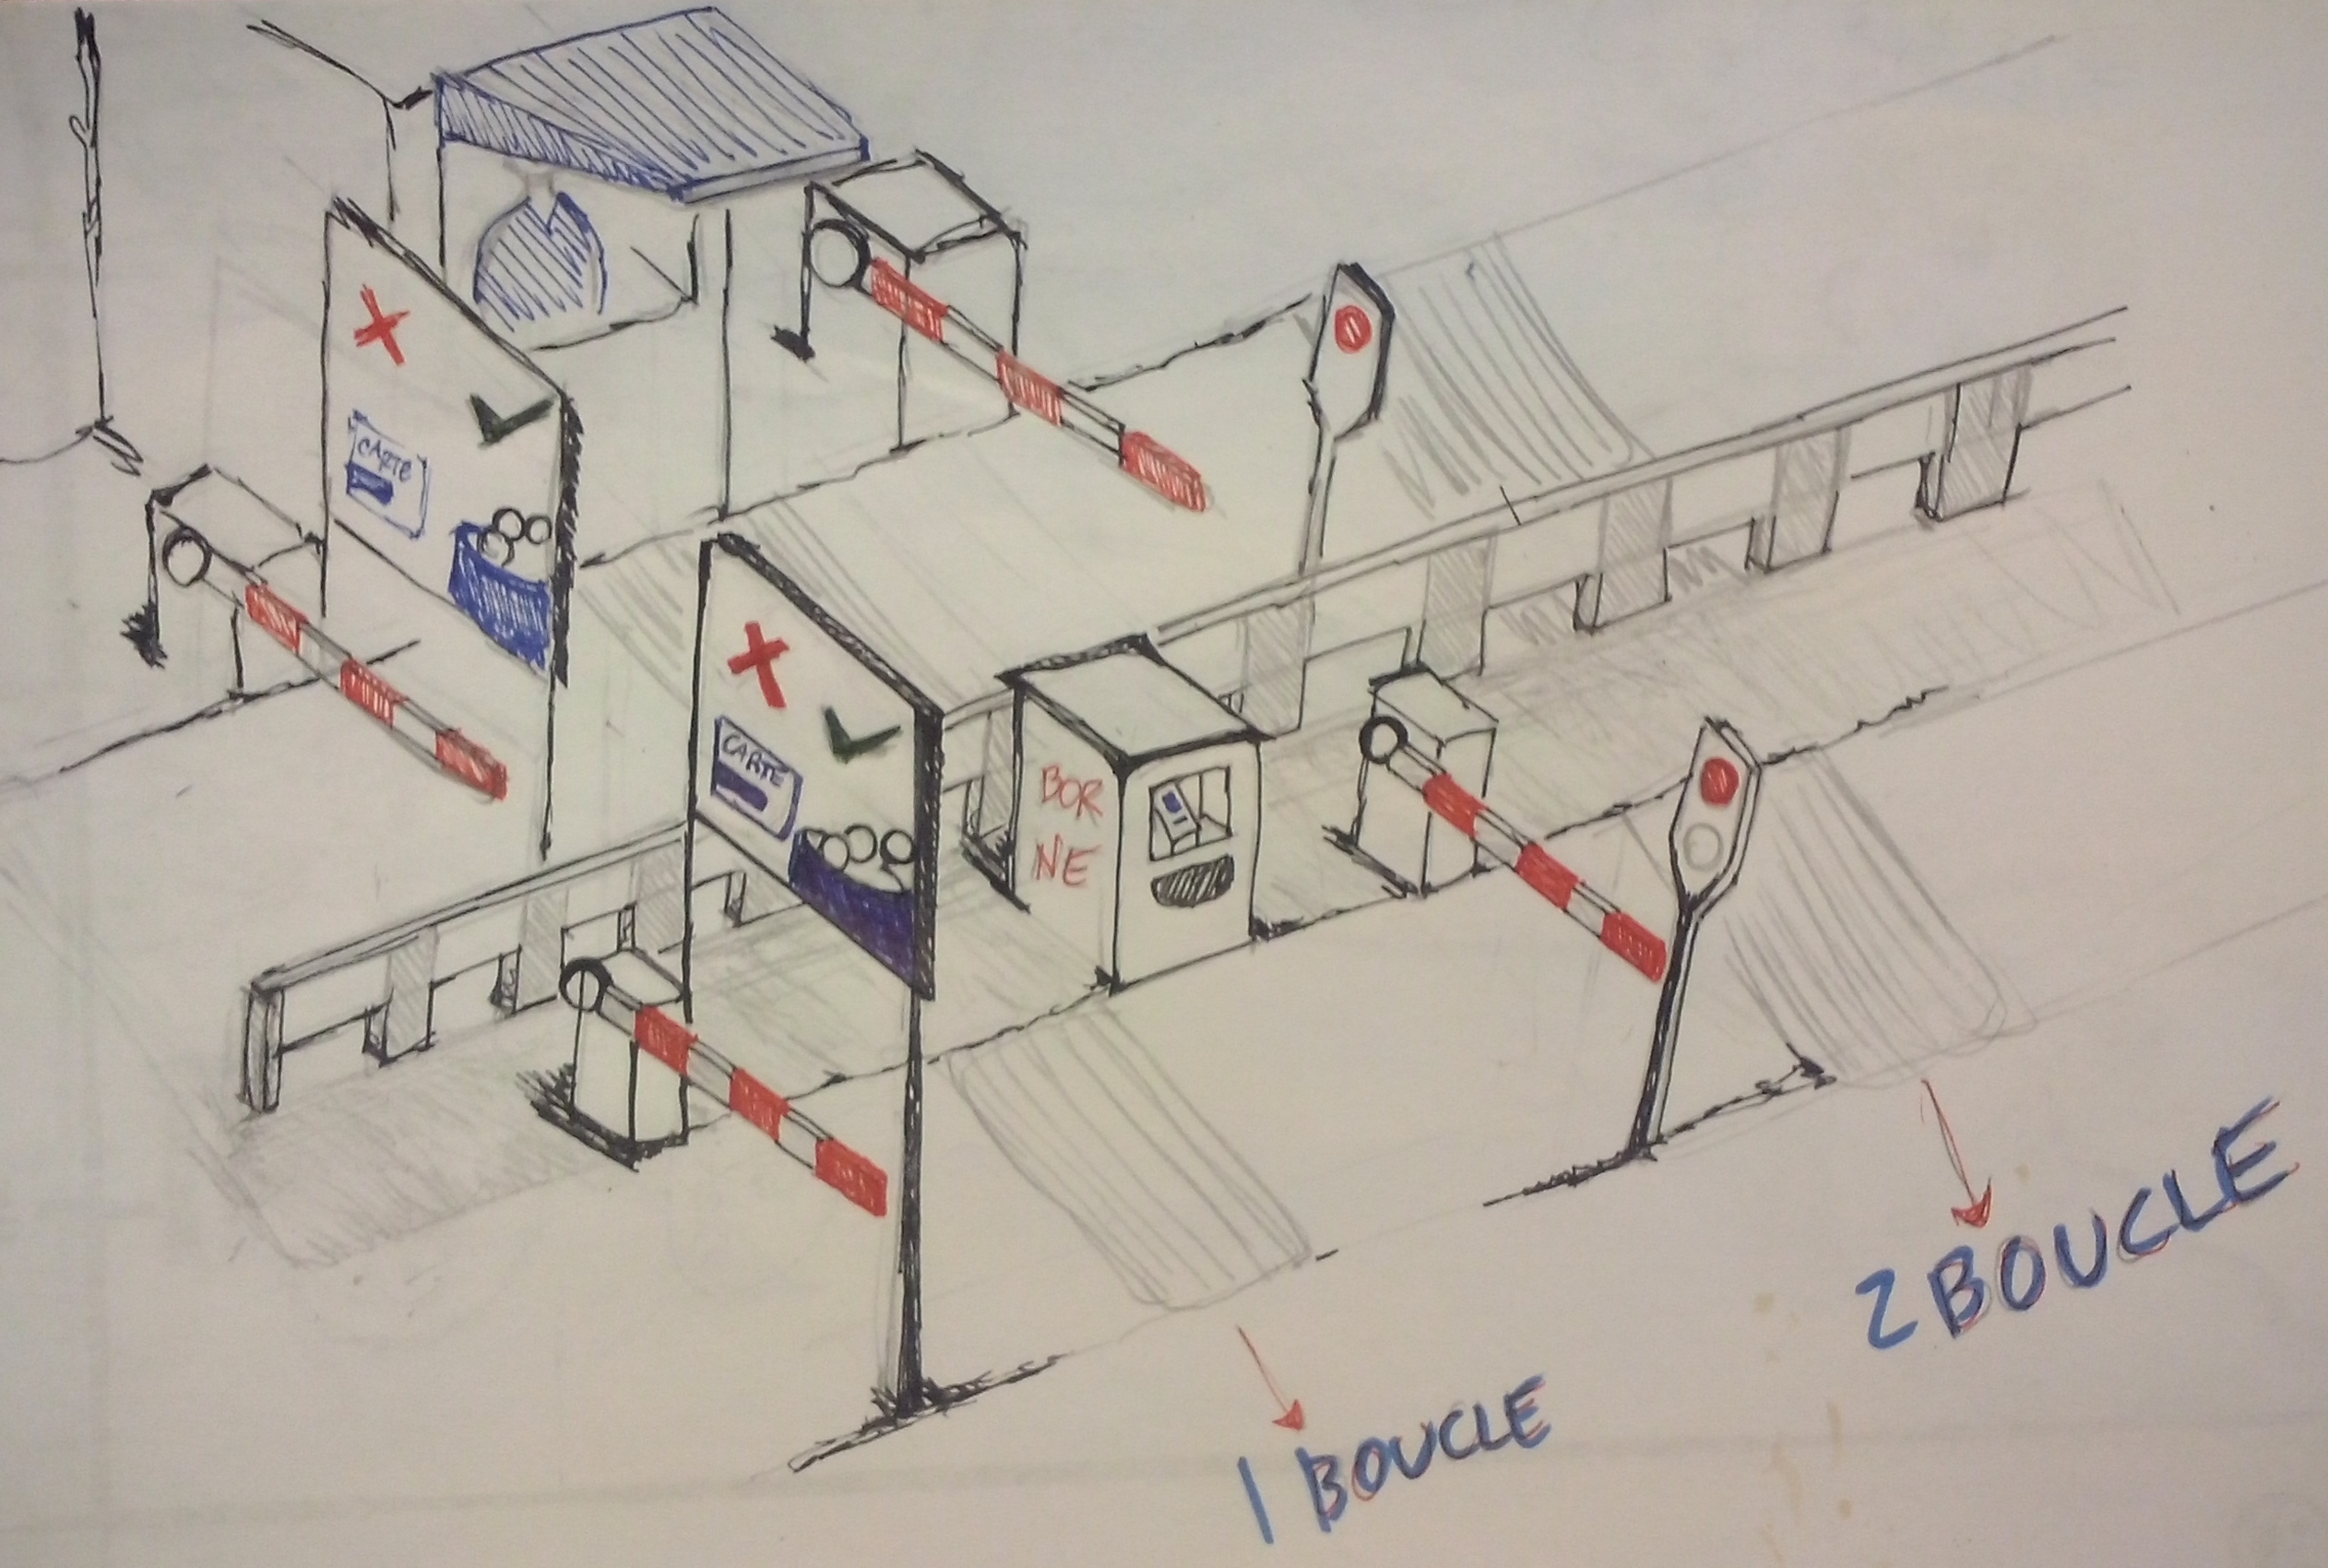
\includegraphics[scale=0.16]{02_Desenvolvimento/TD1/images/desc.png}
    \caption{Description physique}
    \label{fig:my_label}
\end{figure}
\newpage
\section{Réécriture de l'expression des besoins recentrée sur les utilisateurs du systeme}
\subsection{Les acteurs} 
Nous avons reconnu cinq acteurs (utilisateurs) du système tel que :
\begin{itemize}
    \item \textbf{Le Client (Conducteur de voiture)}: Le conducteur est le client, le rôle du conducteur est de passer la barrière de péage autoroutiere. 
    \item \textbf{La Société d’Autoroute}: 	La société est la propriétaire de la barrière de péage et gère donc la barrière. C’est elle qui va gérer aussi les cartes d’abonnement et le traitement des comptes des abonnés. 
    \item \textbf{Le Technicien}: Le technicien est l’acteur premier pour la maintenance du système. Le technicien lève la barrière manuellement en cas d’urgence. Il va faire des interventions humaines si necessaire, ex: si la barrière ne s’ouvre pas. 
    \item \textbf{Operateur humain}: L’ operateur humain reçoit le paiement du client (conducteur) dans les bornes manuelles.
    \item \textbf{Le Surveillant}: Les surveillants supervisent l’ensemble des bornes pour assurer, par exemple, qu’à tout moment il y ait une voie ouverte ou que le nombre de voies ouvertes soit proportionnel au flux de véhicules. Si le système lève une alarme vers l’ordinateur du poste de surveillance, un surveillant doit faire une intervention, comme remettre de la monnaie dans une borne et fait un compte-rendu approximatif de l’incident.
\end{itemize}
\newpage
\subsection{Les Grandes Fonctionnalités du Système}
Nous avons différencié trois grandes fonctionnalités du système:\\

\textbf{Passer le péage }(\ref{subsubsec:passerL})

\textbf{Gerer la comptapilité } (\ref{subsubsec:gerer})

\textbf{Maintenance }(\ref{subsubsec:maint})\\

Ainsi voici les scénarios informels correspondant :
\subsubsection{\textbf{Cas d’utilisation:} Passer le péage } \label{subsubsec:passerL} 
\textbf{Acteur primaire}: Le Client (le conducteur) 

\textbf{Acteur support}: La Société d’Autoroute, le technicien, l’operateur humain et le surveillant

Le client (le conducteur) opte pour une voie selon son type de véhicule et le moyen de paiement. Le client effectue le paiement selon le type de borne qu’ il a choisi (avec une carte d’abonnement, carte de crédit, monnaie, monnaie avec un opérateur humain, etc). Le système gère l’ouverture de la barrière une fois le montant payé ou la carte d’abonnement présenté, si la barrière ne s’ouvre pas, alors un technicien ou un opérateur doit venir régler l’incident survenu.


\subsubsection{\textbf{Cas d’utilisation:} Gerer la comptabilité}  \label{subsubsec:gerer}
\textbf{Acteur primaire}: La Société d'autoroute 

Le système doit assurer la comptabilité générale de l’ensemble des bornes. Chaque levée de barrière est enregistré. Les cartes d’abonnement et les compte des abonnés sont gérés par la société d’autoroute de façon instantanée, chaque passage est enregistré. Les opérations par cartes bleues sont gérées en fin de journée. Les bornes détectent les fausses pièces et les cartes volées.

\subsubsection{\textbf{Cas d’utilisation:} Maintenance}  \label{subsubsec:maint}
\textbf{Acteur primaire}: Le Technicien 

\textbf{Acteur support}: Le surveillant, l’opérateur humain

Le technicien permet de gérer toutes les cas, incidents, qui nécessitent une intervention humaine, lorsque qu’une barrière doit être ouverte ou fermée manuellement, lorsqu’un usager se retrouve coincé à la barrière de péage ou lorsqu’une borne a besoin de réglage ou de réparation (comme remettre de la monnaie).



\mychapter{TD2}
\label{Cap:TD2}

\section{Diagramme UC de haut niveau}
\begin{figure}[h]
    \centering
    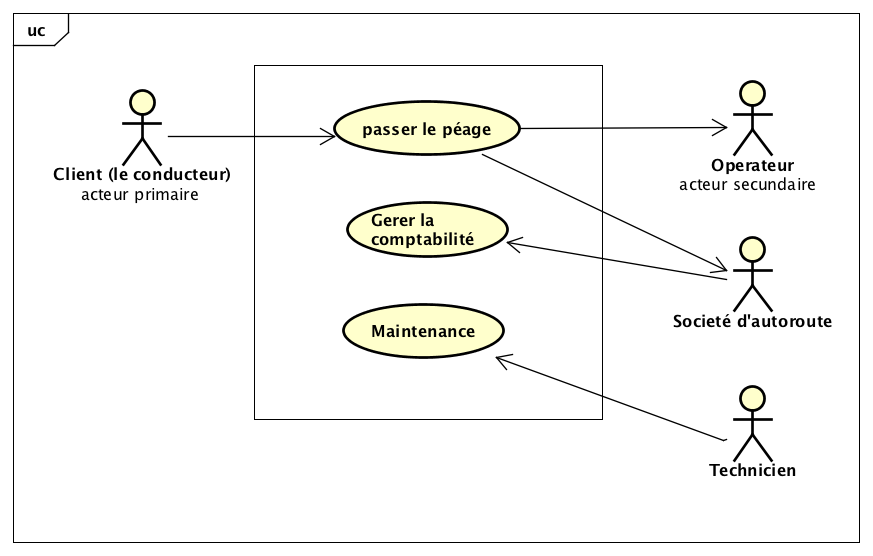
\includegraphics[scale=0.55]{images/hautNiveau.png}
    \caption{Diagramme de haut niveau - Passer le péage}
    \label{fig:my_label}
\end{figure}
\newpage
\section{Scenários Cockburn - Passer le péage}\label{sec:passer}
    \textbf{Cas d'utilisation:} Passer le péage
    
    \textbf{Acteur primaire (initiateur):} Conducteur
    
    \textbf{Acteur support:} -
    
    \textbf{Pré-condition: } nécessite que la voie soit ouverte.
    
    \textbf{Post-condition: }   la voie redevient disponible(ouverte et libre) pour un prochain usager.
    
    \textbf{Scenario primaire: } \\
    \textbf{1.} L’usager rentre dans la voie d’autoroute. \\
    \textbf{2.} L’usager paie le passage (\ref{subsec:paie})\\
    \textbf{3.} L’usager passe.
    
    \textbf{Variantes}\\
    \textbf{3a.} L'usager ne passe pas : la barrière reste ouverte en attendant la sortie de l’usager.

\section{Scenários Secundaries}
\subsection{Scenários Cockburn - Paie le passage} \label{subsec:paie}
\textbf{Cas d'utilisation:}

\textbf{Acteur primaire:}Paie le passage Conducteur

\textbf{Acteur support:} le poste de surveillance et opérateur humain(si le borne est manuelle)

\textbf{Pré-condition: } La boucle au sol détermine la présence du véhicule
 
\textbf{Post-condition: } 

\textbf{Scenario primaire: } \\
    \textbf{1.} Paier pour carte bancaire\\
    \textbf{2.} Paier avec argent\\
    \textbf{3.} Paier avec cart abonnement\\

\textbf{Variantes:}\\
    \textbf{2a.} Verifier pièces %Se algo é feito automatico eu devo escrever? ps2: se é so feito pela borne automatique, como escrevo condicao? 
\subsection{Scenários Cockburn} \label{subsec:}
\textbf{Cas d'utilisation:}

\textbf{Acteur primaire:}

\textbf{Acteur support:}

\textbf{Pré-condition: } 
 
\textbf{Post-condition: } 

\textbf{Scenario primaire: } \\
    \textbf{1.} \\
    \textbf{2.} \\
    \textbf{3.}

\textbf{Variantes:}\\
    \textbf{2a.} 
\newpage
\section*{Diagrammé UC détaillés}
\begin{figure}[h]
    \centering
    %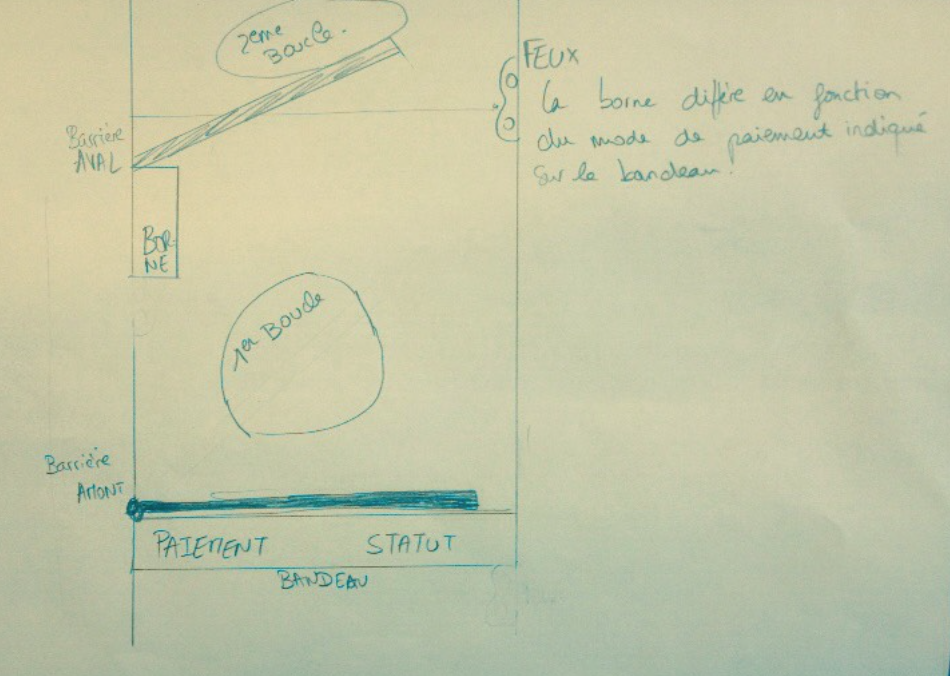
\includegraphics[scale=0.9]{a.png}
    \caption{Diagrammé UC détaillés - passage}
    \label{fig:my_label}
\end{figure} 


\mychapter{Réécriture}
\label{Cap:TD1}


\section{Description physique}
Nous avons perçu que le système demandé sur la gestion d’une voie de péage d’autoroute.
%Nous avons élaborré dans ce document une première description de système d’un péage d’autoroute.

\begin{figure}[h]
    \centering
    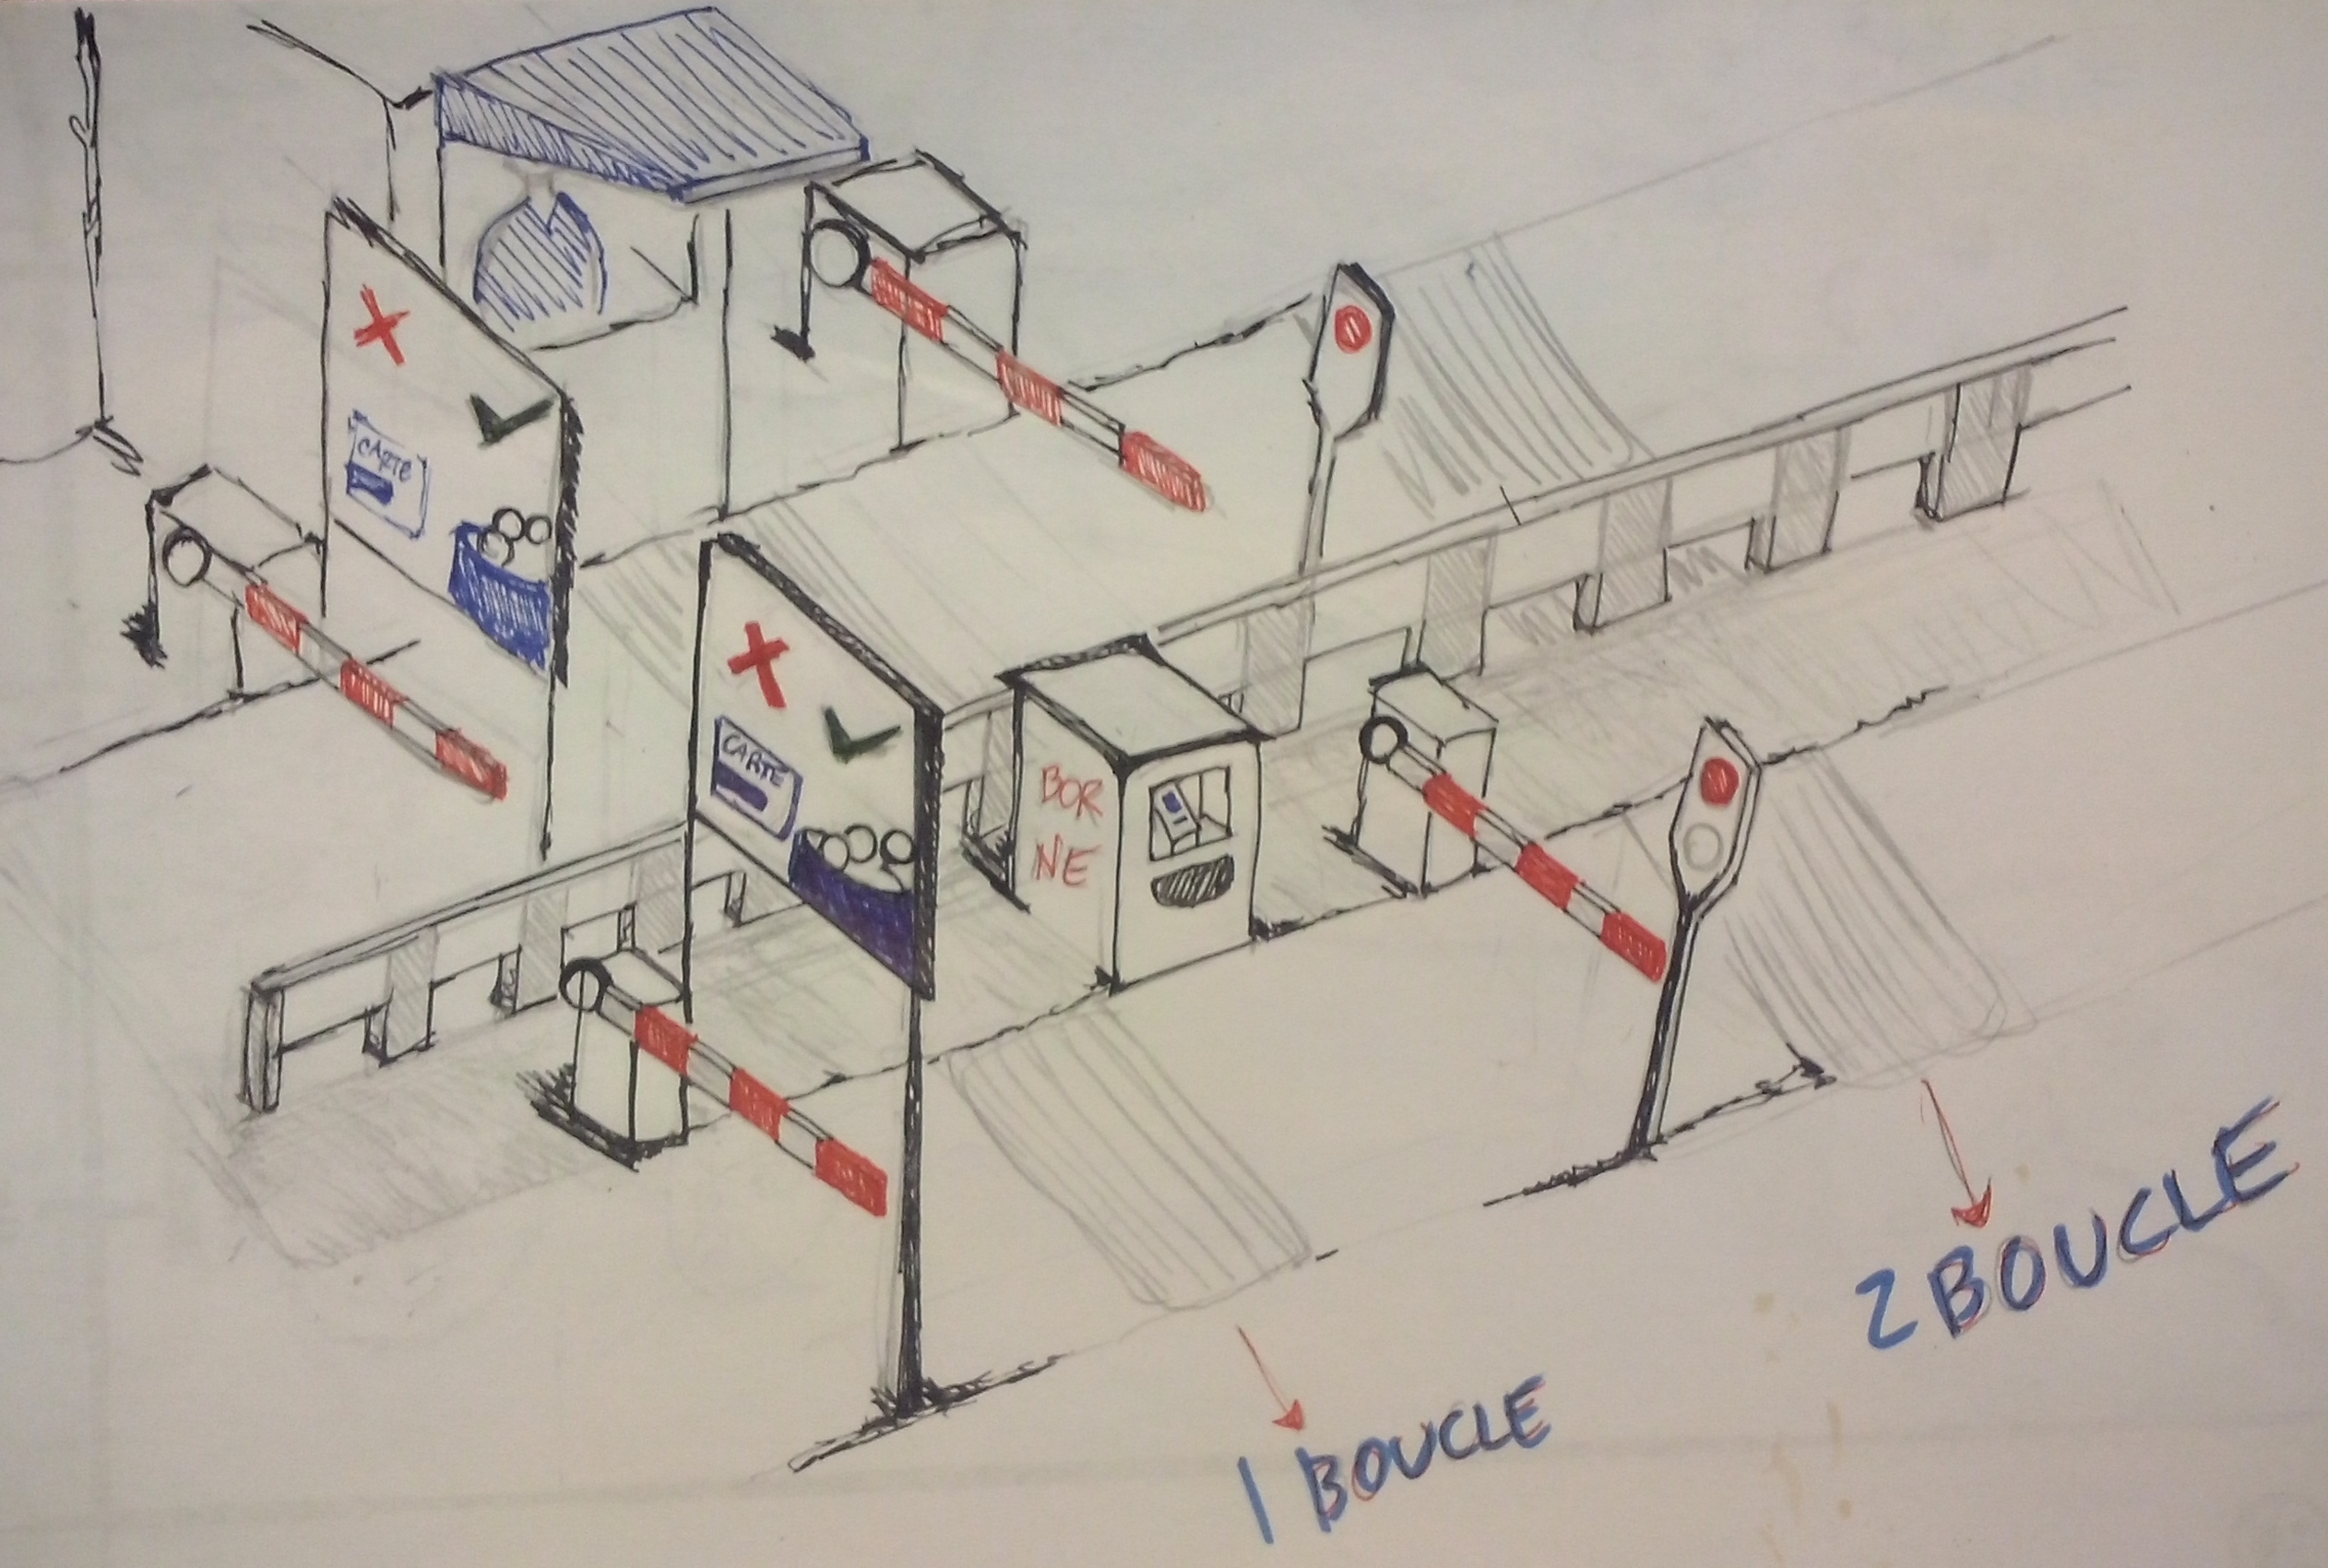
\includegraphics[scale=0.16]{02_Desenvolvimento/TD1/images/desc.png}
    \caption{Description physique}
    \label{fig:my_label}
\end{figure}
\newpage
\section{Réécriture de l'expression des besoins recentrée sur les utilisateurs du systeme}
\subsection{Les acteurs} 
Nous avons reconnu cinq acteurs (utilisateurs) du système tel que :
\begin{itemize}
    \item \textbf{Le Client (Conducteur de voiture)}: Le conducteur est le client, le rôle du conducteur est de passer la barrière de péage autoroutiere. 
    \item \textbf{La Société d’Autoroute}: 	La société est la propriétaire de la barrière de péage et gère donc la barrière. C’est elle qui va gérer aussi les cartes d’abonnement et le traitement des comptes des abonnés. 
    \item \textbf{Le Technicien}: Le technicien est l’acteur premier pour la maintenance du système. Le technicien lève la barrière manuellement en cas d’urgence. Il va faire des interventions humaines si necessaire, ex: si la barrière ne s’ouvre pas. 
    \item \textbf{Operateur humain}: L’ operateur humain reçoit le paiement du client (conducteur) dans les bornes manuelles.
    \item \textbf{Le Surveillant}: Les surveillants supervisent l’ensemble des bornes pour assurer, par exemple, qu’à tout moment il y ait une voie ouverte ou que le nombre de voies ouvertes soit proportionnel au flux de véhicules. Si le système lève une alarme vers l’ordinateur du poste de surveillance, un surveillant doit faire une intervention, comme remettre de la monnaie dans une borne et fait un compte-rendu approximatif de l’incident.
\end{itemize}
\newpage
\subsection{Les Grandes Fonctionnalités du Système}
Nous avons différencié trois grandes fonctionnalités du système:\\

\textbf{Passer le péage }(\ref{subsubsec:passerL})

\textbf{Gerer la comptapilité } (\ref{subsubsec:gerer})

\textbf{Maintenance }(\ref{subsubsec:maint})\\

Ainsi voici les scénarios informels correspondant :
\subsubsection{\textbf{Cas d’utilisation:} Passer le péage } \label{subsubsec:passerL} 
\textbf{Acteur primaire}: Le Client (le conducteur) 

\textbf{Acteur support}: La Société d’Autoroute, le technicien, l’operateur humain et le surveillant

Le client (le conducteur) opte pour une voie selon son type de véhicule et le moyen de paiement. Le client effectue le paiement selon le type de borne qu’ il a choisi (avec une carte d’abonnement, carte de crédit, monnaie, monnaie avec un opérateur humain, etc). Le système gère l’ouverture de la barrière une fois le montant payé ou la carte d’abonnement présenté, si la barrière ne s’ouvre pas, alors un technicien ou un opérateur doit venir régler l’incident survenu.


\subsubsection{\textbf{Cas d’utilisation:} Gerer la comptabilité}  \label{subsubsec:gerer}
\textbf{Acteur primaire}: La Société d'autoroute 

Le système doit assurer la comptabilité générale de l’ensemble des bornes. Chaque levée de barrière est enregistré. Les cartes d’abonnement et les compte des abonnés sont gérés par la société d’autoroute de façon instantanée, chaque passage est enregistré. Les opérations par cartes bleues sont gérées en fin de journée. Les bornes détectent les fausses pièces et les cartes volées.

\subsubsection{\textbf{Cas d’utilisation:} Maintenance}  \label{subsubsec:maint}
\textbf{Acteur primaire}: Le Technicien 

\textbf{Acteur support}: Le surveillant, l’opérateur humain

Le technicien permet de gérer toutes les cas, incidents, qui nécessitent une intervention humaine, lorsque qu’une barrière doit être ouverte ou fermée manuellement, lorsqu’un usager se retrouve coincé à la barrière de péage ou lorsqu’une borne a besoin de réglage ou de réparation (comme remettre de la monnaie).



\mychapter{TD2}
\label{Cap:TD2}

\section{Diagramme UC de haut niveau}
\begin{figure}[h]
    \centering
    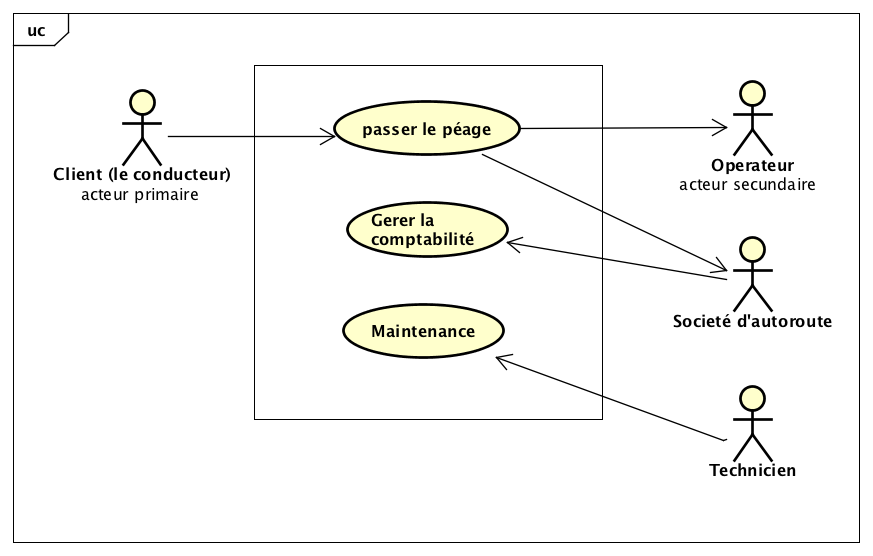
\includegraphics[scale=0.55]{images/hautNiveau.png}
    \caption{Diagramme de haut niveau - Passer le péage}
    \label{fig:my_label}
\end{figure}
\newpage
\section{Scenários Cockburn - Passer le péage}\label{sec:passer}
    \textbf{Cas d'utilisation:} Passer le péage
    
    \textbf{Acteur primaire (initiateur):} Conducteur
    
    \textbf{Acteur support:} -
    
    \textbf{Pré-condition: } nécessite que la voie soit ouverte.
    
    \textbf{Post-condition: }   la voie redevient disponible(ouverte et libre) pour un prochain usager.
    
    \textbf{Scenario primaire: } \\
    \textbf{1.} L’usager rentre dans la voie d’autoroute. \\
    \textbf{2.} L’usager paie le passage (\ref{subsec:paie})\\
    \textbf{3.} L’usager passe.
    
    \textbf{Variantes}\\
    \textbf{3a.} L'usager ne passe pas : la barrière reste ouverte en attendant la sortie de l’usager.

\section{Scenários Secundaries}
\subsection{Scenários Cockburn - Paie le passage} \label{subsec:paie}
\textbf{Cas d'utilisation:}

\textbf{Acteur primaire:}Paie le passage Conducteur

\textbf{Acteur support:} le poste de surveillance et opérateur humain(si le borne est manuelle)

\textbf{Pré-condition: } La boucle au sol détermine la présence du véhicule
 
\textbf{Post-condition: } 

\textbf{Scenario primaire: } \\
    \textbf{1.} Paier pour carte bancaire\\
    \textbf{2.} Paier avec argent\\
    \textbf{3.} Paier avec cart abonnement\\

\textbf{Variantes:}\\
    \textbf{2a.} Verifier pièces %Se algo é feito automatico eu devo escrever? ps2: se é so feito pela borne automatique, como escrevo condicao? 
\subsection{Scenários Cockburn} \label{subsec:}
\textbf{Cas d'utilisation:}

\textbf{Acteur primaire:}

\textbf{Acteur support:}

\textbf{Pré-condition: } 
 
\textbf{Post-condition: } 

\textbf{Scenario primaire: } \\
    \textbf{1.} \\
    \textbf{2.} \\
    \textbf{3.}

\textbf{Variantes:}\\
    \textbf{2a.} 
\newpage
\section*{Diagrammé UC détaillés}
\begin{figure}[h]
    \centering
    %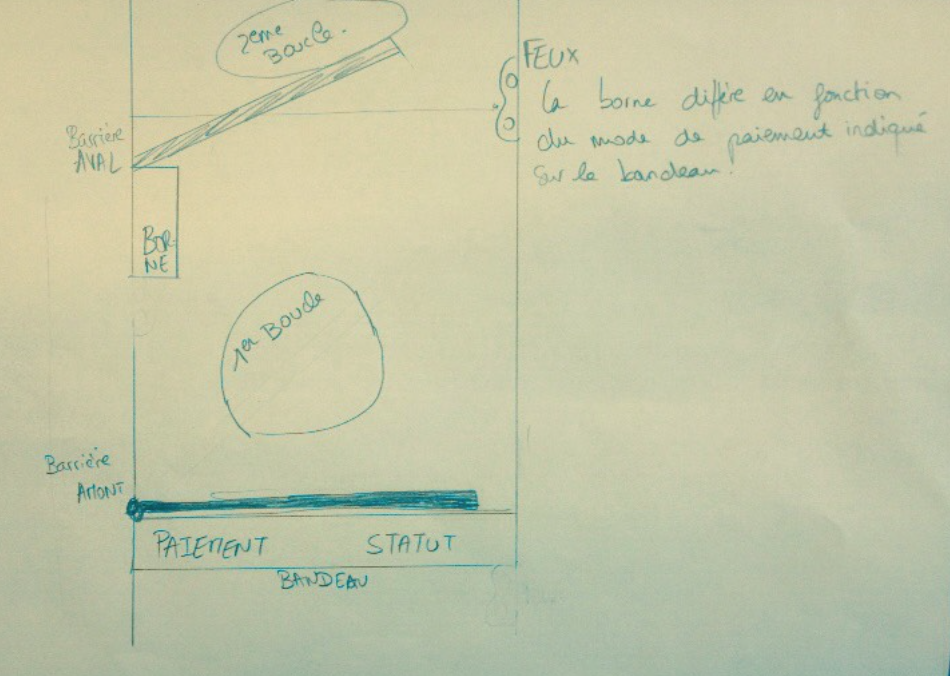
\includegraphics[scale=0.9]{a.png}
    \caption{Diagrammé UC détaillés - passage}
    \label{fig:my_label}
\end{figure} 

% Conclus�es
%%%
%% Cap�tulo 5: Conclus�es
%%

\mychapter{Conclusão}
\label{Cap:conclusao} 
%%%
%% Cap�tulo 5: Conclus�es
%%

\mychapter{Conclusão}
\label{Cap:conclusao} 

\backmatter

%\chapter{Anexos}


% Refer�ncias bibliog�ficas (geradas automaticamente)
%\bibliographystyle{ppgee}

%\bibliographystyle{dcu}
%\addcontentsline{toc}{chapter}{Referências bibliográficas}

%Arquivo com as bibliografias
%\bibliography{bibliografia}


\end{document}
